\noindent\textbf{About this recipe:}\\
This recipe will provide you with delicious and fluffy naan bread.
While traditional naan bread is not leavened and made with the help of
a hot Tandoor oven, this recipe is tailored to be made with your
home oven setup.

This recipe takes around 2 hours to complete when opting for the yeast based
dough. When using the sourdough option replace the yeast with around 10
percent sourdough starter based on the flour. The sourdough option will take
longer to bulkferment but will present superb slightly tangy tasting naans.

\begin{figure}[h]
    \centering
    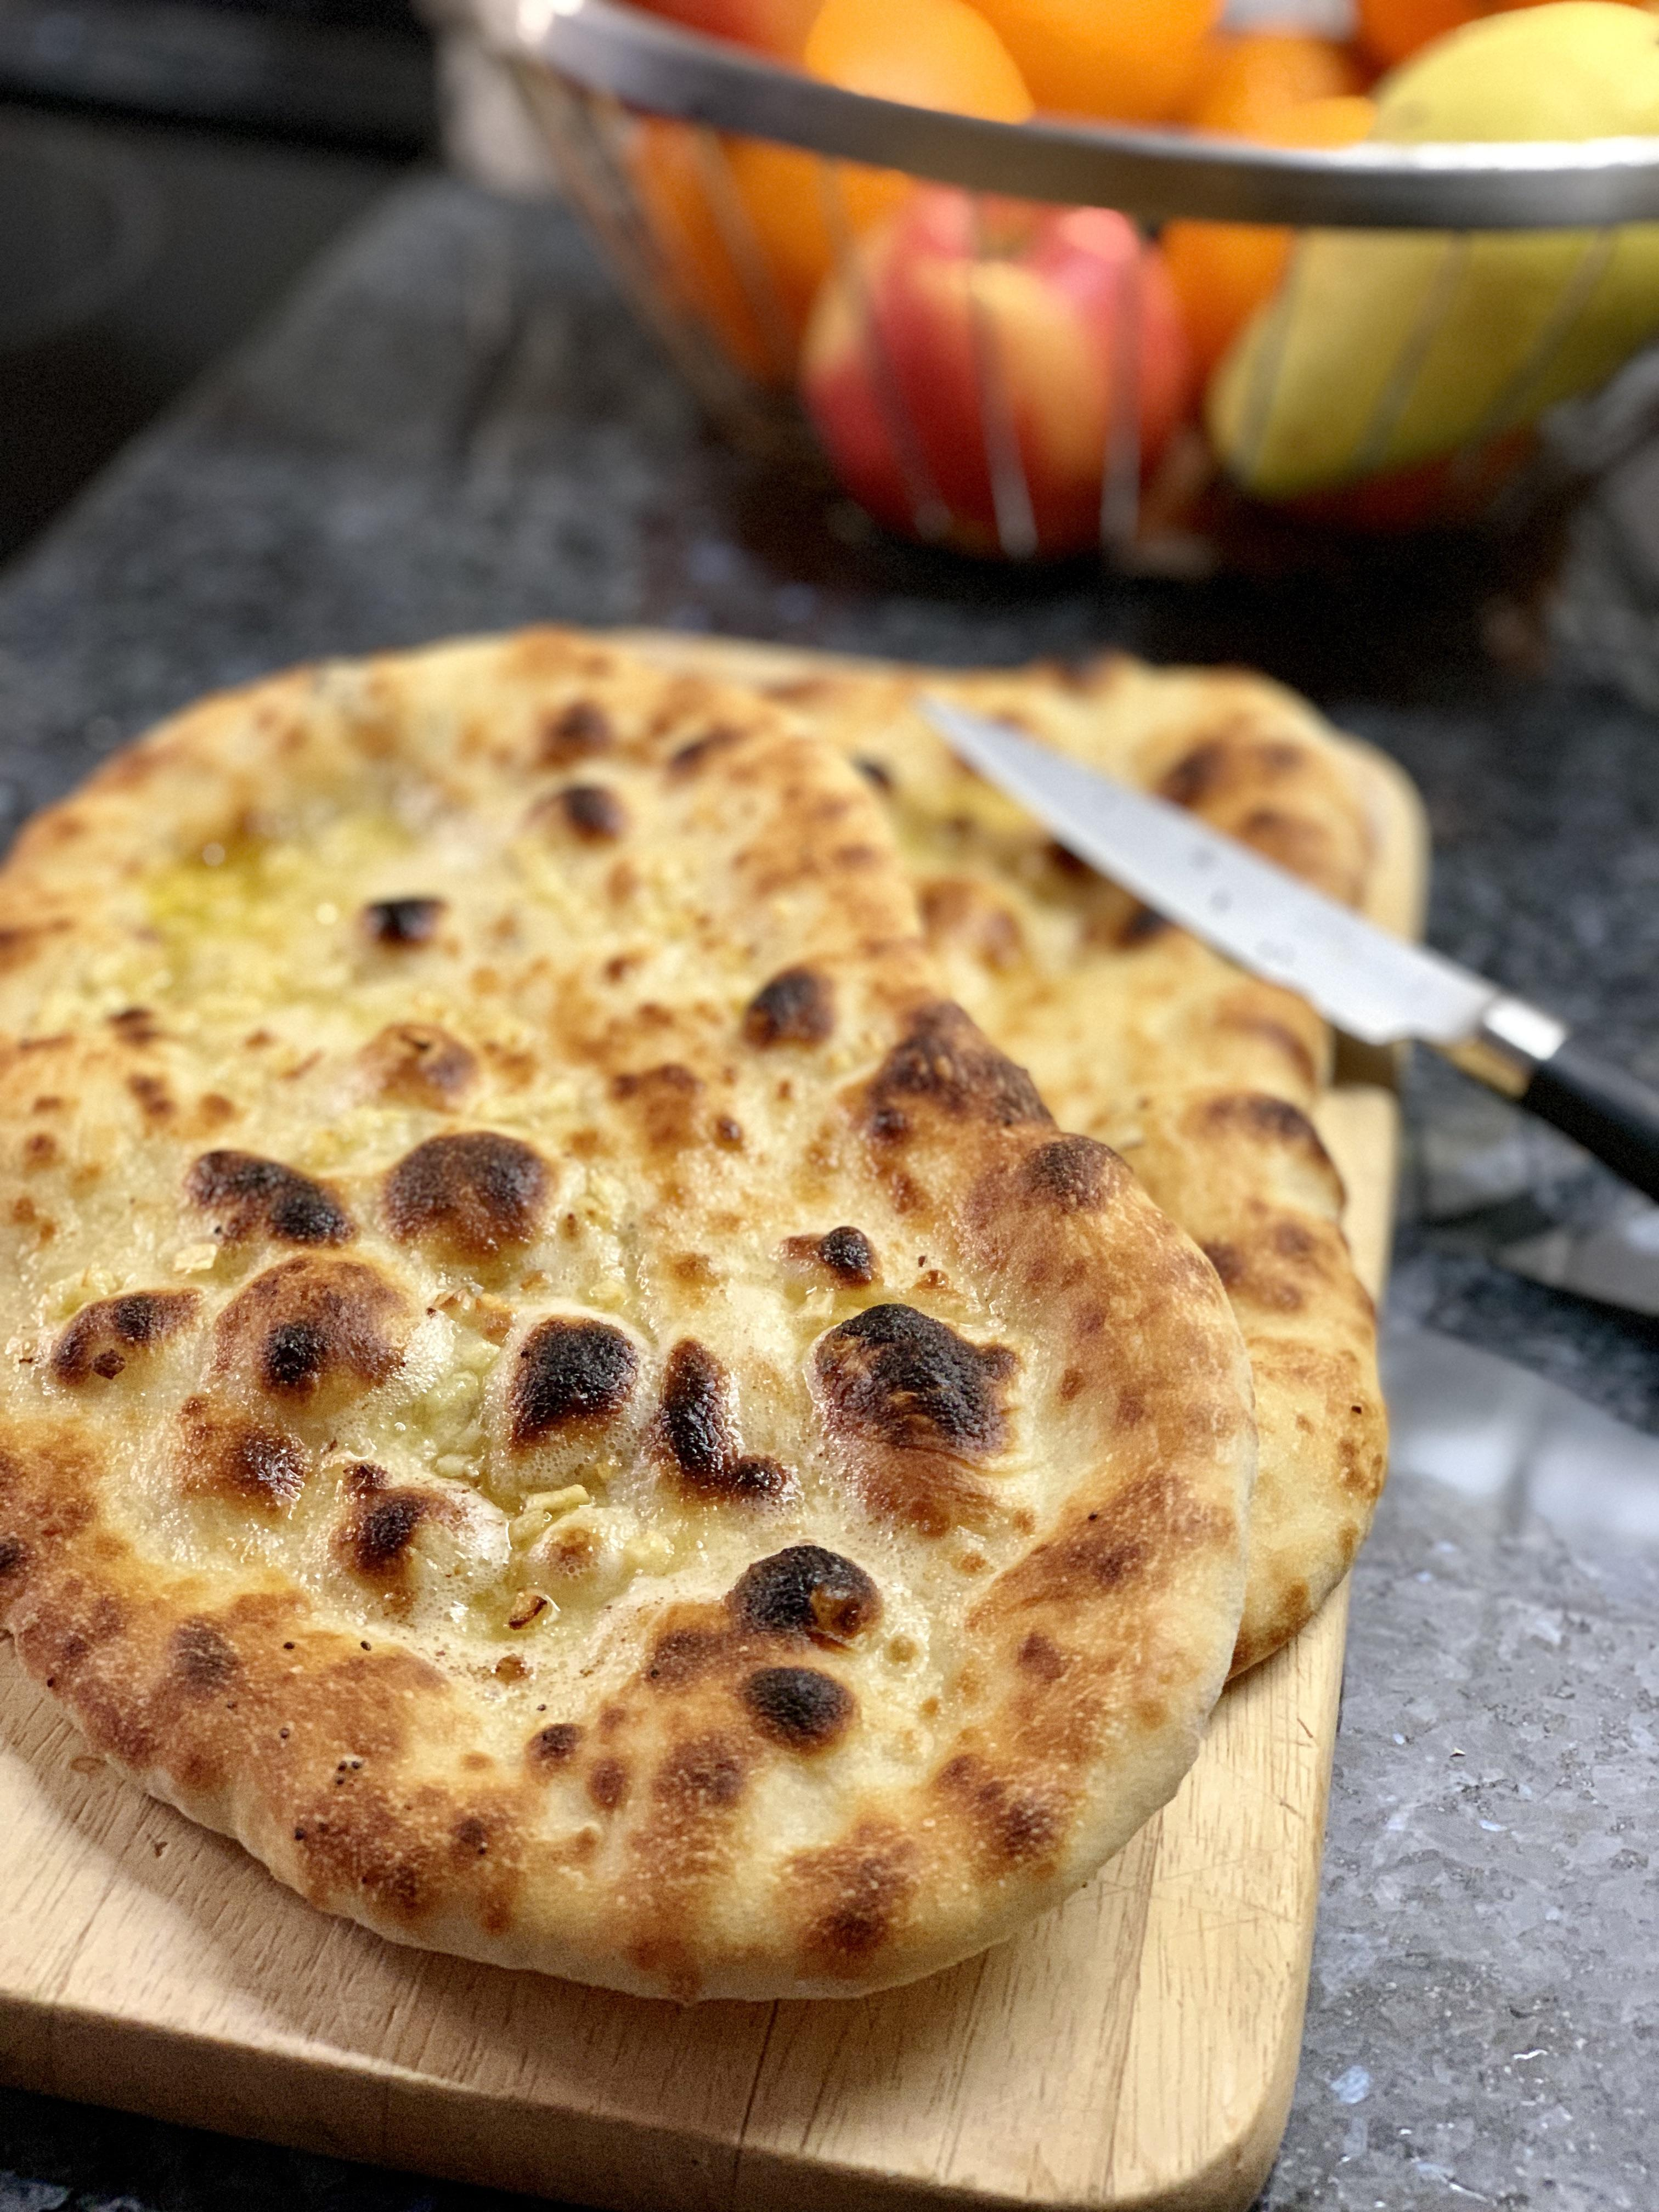
\includegraphics[width=0.6\textwidth]{naan}
    \caption{Fluffy naans topped with garlic butter}
\end{figure}

\noindent\textbf{Ingredients:}

\begin{center}
\begin{tabular}{|c|l|r|r|}
    \hline
    \textbf{No.} & \textbf{Ingredient} & \textbf{Quantity} & \textbf{Baker's math} \\
    \hline
    1 & All purpose flour & 400 g = 4 pieces & 100\% \\
    \hline
    2 & Water, warm & 160 g & 40\% \\
    \hline
    3 & Yogurt & 160 g & 40\% \\
    \hline
    4 & Butter & 40 g & 10\% \\
    \hline
    5 & Sugar & 12 g & 3\% \\
    \hline
    6 & Salt & 8 g & 2\% \\
    \hline
    7 & Sourdough starter & 40 g & 10\% \\
    \hline
\end{tabular}
\end{center}

\noindent\textbf{Instructions:}
\begin{center}
\begin{tabular}{|c|p{12cm}|}
    \hline
    \textbf{Step} & \textbf{Instruction} \\
    \hline
    1 & Mix everything together. No need to heavily knead. Just stir it with
    your hands. Let it rest for 20 minutes. This will help the gluten to
    develop. Add the butter directly. The dough should not be too wet,
    if you feel it is too sticky, proceed and add more flour. Make sure
    to create a smooth dough ball before proceeding. \\
    \hline
    2 & Stretch and fold if you see the dough flattened out a lot \\
    \hline
    3 & Wait 30~minutes (different for sourdough) \\
    \hline
    4 & Stretch and fold if you see the dough flattened out a lot \\
    \hline
    5 & Wait until the dough is doubled in size, preshape into equally portioned
    dough balls For the sourdough option aim for a 50\% size increase \\
    \hline
    6 & Preheat oven to max temperature for around 30~minutes \\
    \hline
\end{tabular}
\end{center}

\noindent\textbf{Baking:}
\begin{center}
\begin{tabular}{|c|p{12cm}|}
    \hline
    \textbf{Step} & \textbf{Instruction} \\
    \hline
    1 & Stretch dough balls with hands. Use flour to make it non stick. Try to
    degas the dough balls as little as possible while stretching. Similar to
    making a pizza. \\
    \hline
    2 & Place naans on rack, stone or steel. Optional: Cover naans with melted
    butter and garlic mixture. \\
    \hline
    3 & Bake until golden brown. Eat while still hot, or wrap in towel to
    preserve moisture if eating later. When eating next day, rinse with water
    and heat again in oven. \\
    \hline
\end{tabular}
\end{center}

It is essential to have as high heat as possible during baking. This will give
the naan it's typical texture. For this reason if you have a broiler activate
it and bake the breads as close to it as possible.

You can also bake the naans in a hot pan. In this case make sure to use a lid
on the pan to ensure even cooking from the evaporating steam. Flip the Naans
once and bake until golden brown. Try to push the naans down a bit after
flipping. This ensures that they bake evenly and do not have too charred
parts.

Another option is to bake the naans on your bbq. Place the Naans on the hot
rack. Flip the Naans once after they can be removed from the rack with a
spatula. Bake until golden brown.

The last option could be to purchase a Tandoor oven and bake it inside of it.
Place the Naans on the hot side of the Tandoor. Wait until they can be removed
from the side. Your naan is done.

\begin{figure}[h]
    \centering
    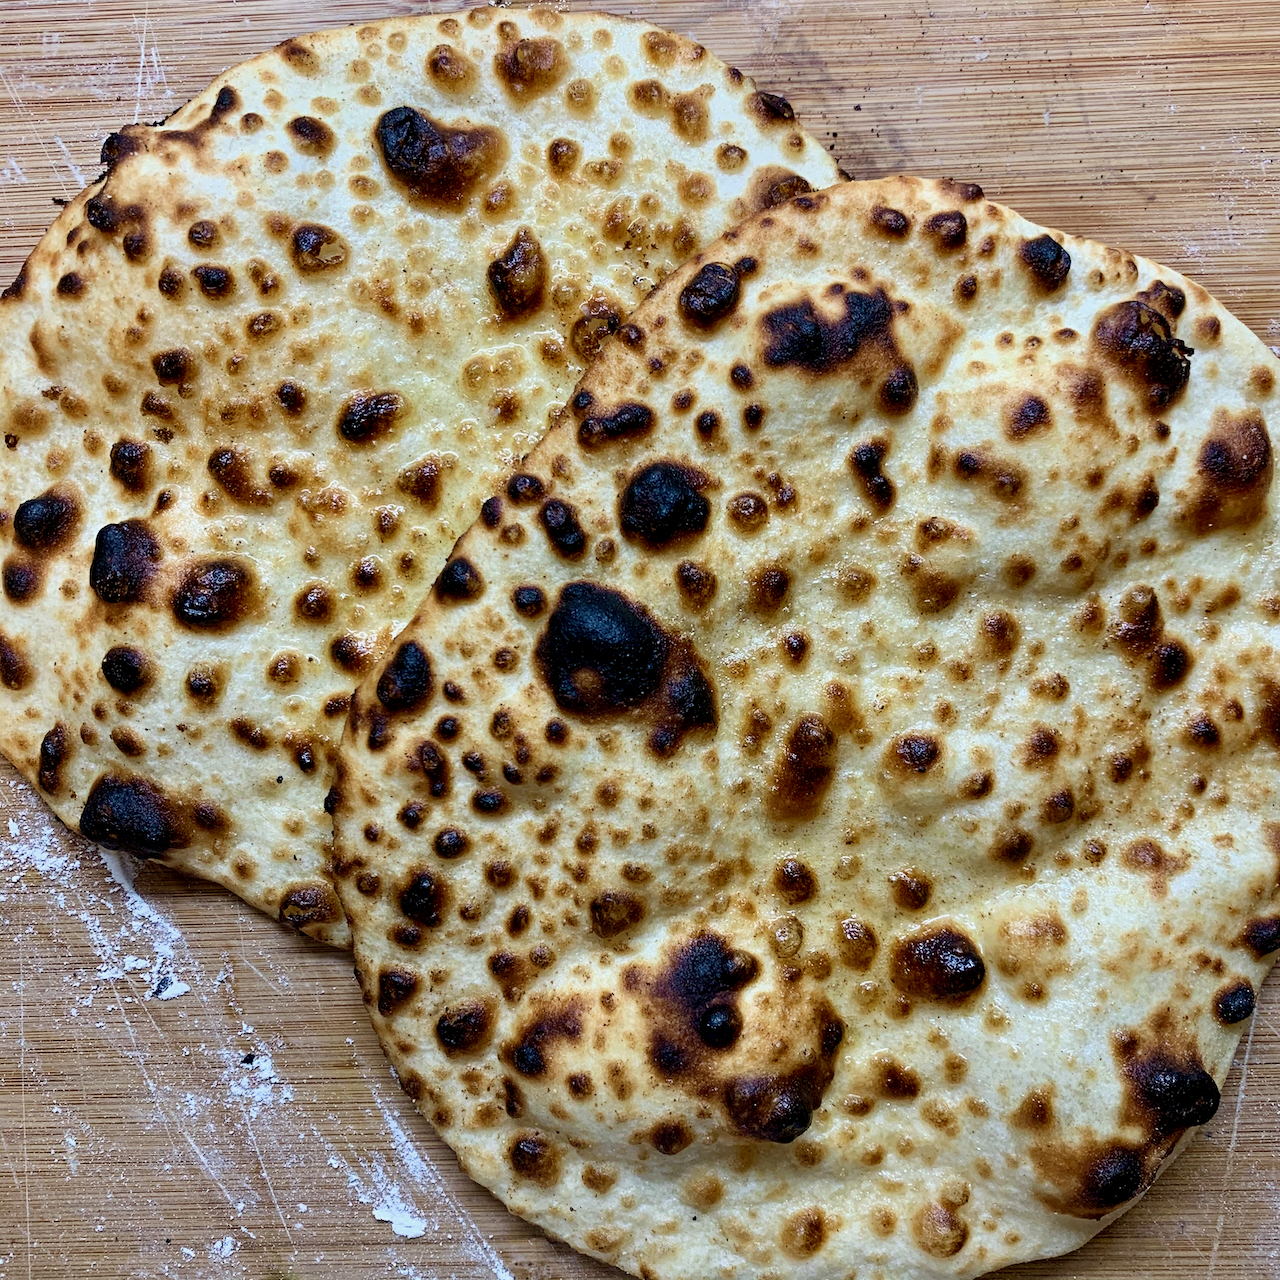
\includegraphics[width=\textwidth]{naan-traditional}
    \caption{Traditional naans are not leavened. The dough only consists of
    flour, water and salt. The dough becomes fluffy due to the hot heat of the
    tandoor oven. In this case, I used a pizza oven to reach 500°C (900°F)}
\end{figure}
